This chapter will review some important considerations when designing and implementing a virtual reality application using gesture recognition as input method.

\section{Virtual Reality hardware}
As described in the previous chapter, a virtual reality head-mounted device (HMD) is in simple terms and device that is fastened to the user's head and, when fastened, covers the
user's entire field of vision. Each eye has its own display, and both of these are positioned about 2-3 centimeters from the eyes. In addition to this several head motion
tracking sensors are built into the headset to detect any movement~\citep{POLYGON2016}. This usually includes a gyroscope, which is responsible for measuring the orientation of the
HMD, and some times an accelerometer to measure the proper acceleration of the HMD \citep{THEVERGE2016}. In addition, or instead of this, the first consumer versions of 
virtual reality headset also usually utilizes some other sensors or cameras outside the HMD. As an example the Oculus Rift CV1 utilizes constellation sensors~\cite{VRFOCUS2015}, 
which are usually positioned on a table, while the HTC Vive utilizes two "lighthouse stations", which are usually placed in opposite corners of the room, and uses photosensors and 
structured light lasers to obtain the users position and rotation~\cite{GIZMODO2015}. 
It is worth noting that both of these virtual reality headset also is sold with their own controllers, which uses similar technology as the HMD, but as previously stated this
thesis will investigate gesture recognition systems as the primary interaction method.  

\begin{figure}%[h!] %[H]
	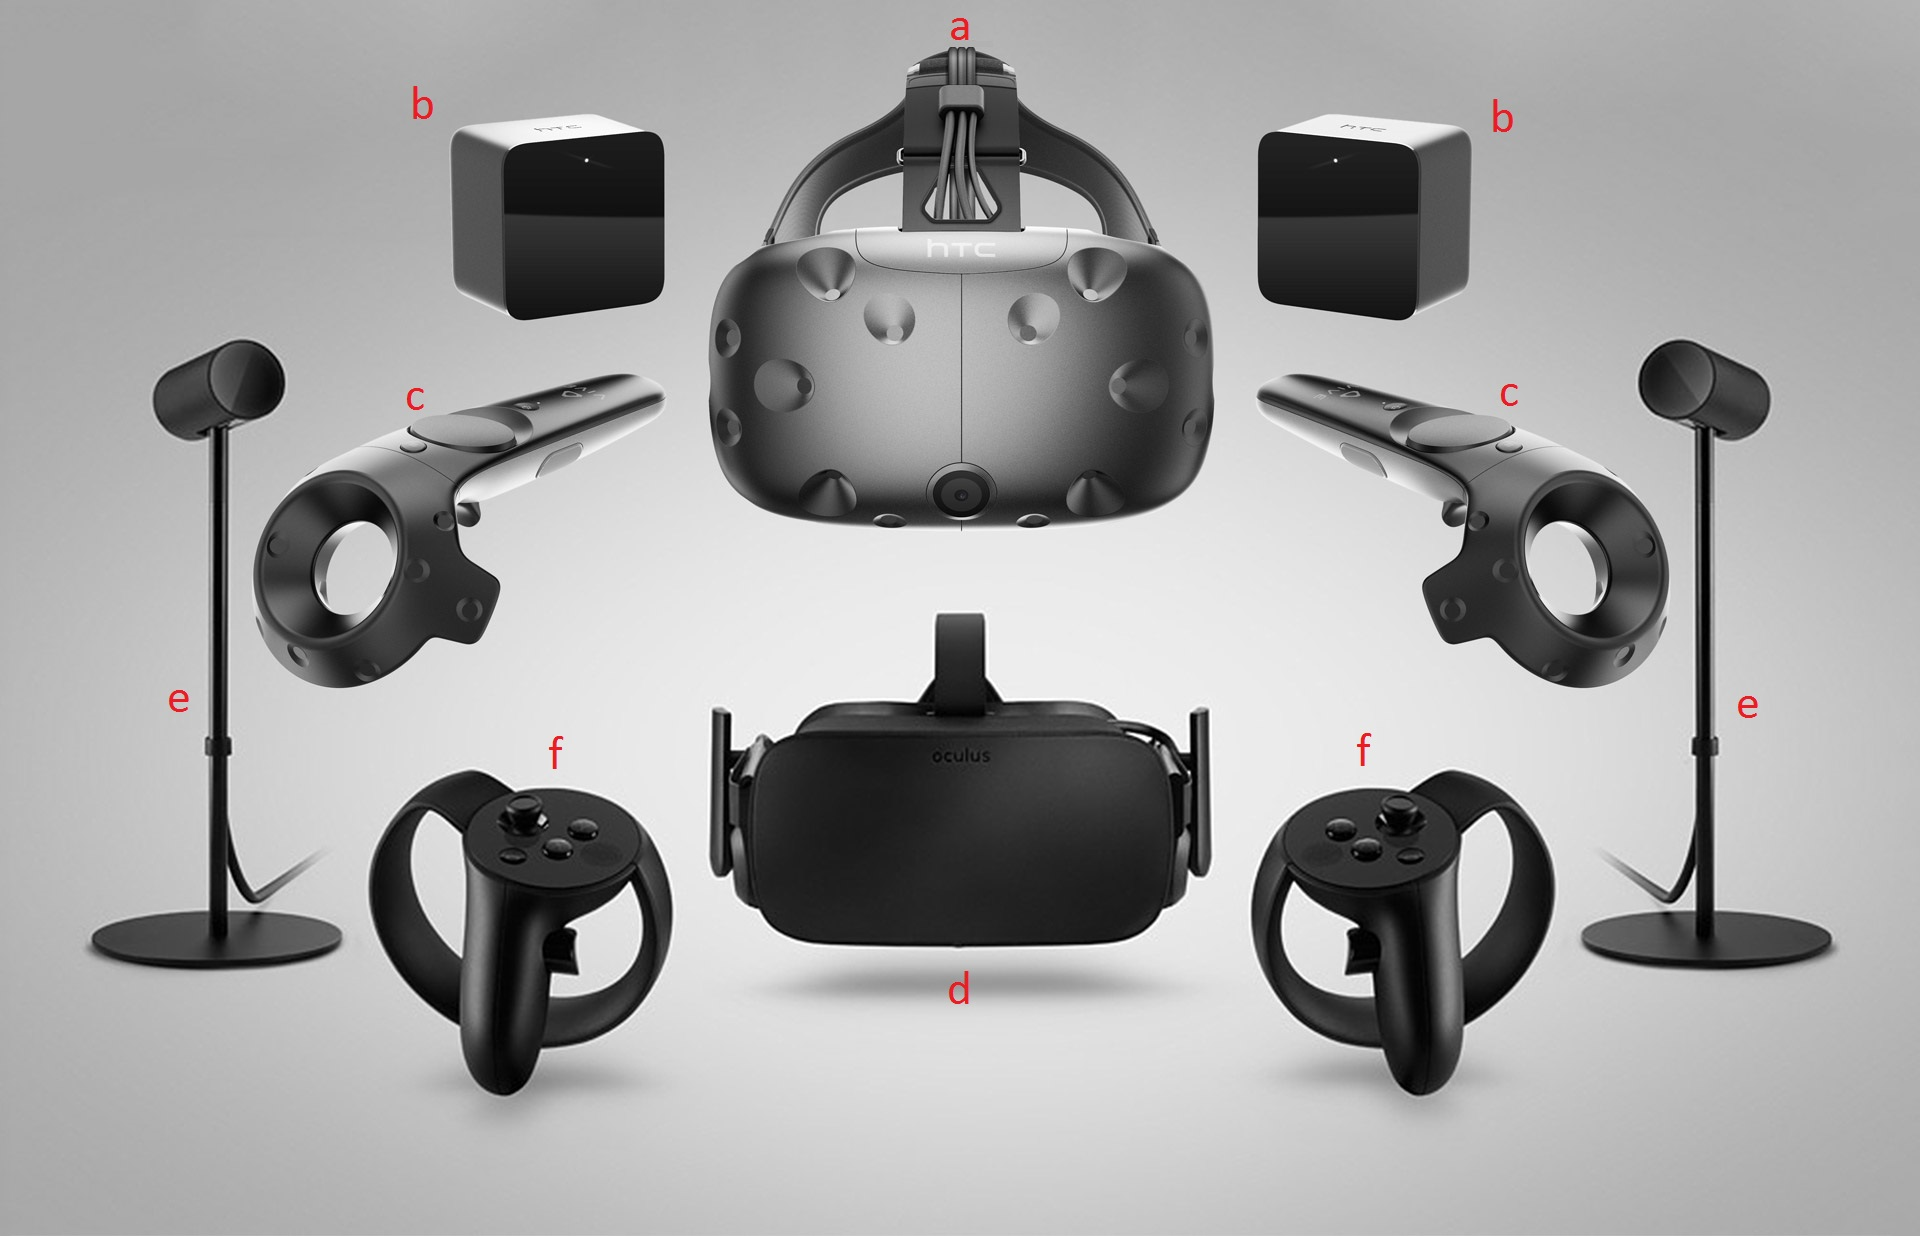
\includegraphics[width=\linewidth]{pictures/vive_and_rift_marked.jpg}
	\caption[The HTC Vive and Oculus Rift Hardware]{The HTC Vive and Oculus Rift Hardware. 
    a) The HTC Vive headset (HMD). b) The HTC Vive Lighthouse Stations. c) The HTC Vive Controllers. d) The Oculus Rift headset (HMD). e) The Oculus Rift Constellation Sensors. 
    f) The Oculus Rift Touch Controllers. Picture from \citet{ROADTOVR2016}}
	\label{fig:vive_and_rift_marked}
\end{figure} 

\section{Virtual reality technical demands}
Virtual reality places some strict demands on performance and software design to avoid discomfort for the user. This is in many ways connected to how virtual reality "tricks" 
the user's brain into thinking the virtual experiences are actually real, thus giving it its "reality feel". Failing to meet these demands can quickly result in significant 
discomfort for the user, often called \textbf{\textit{virtual reality sickness}}, a kind of motion sickness~\citep{ARSTECHNICA2013}. Some of this demands are described below:

\subsection{Latency requirements}
Virtual reality headsets have a much stricter requirements for latency, i.e the time required for an input to have a visible effect, 
than with use of regular displays~\citep{ROADTOVR2013}. If this demand isn't met the system might feel "sluggish", and user's actions and 
visual feedback might feel disjoint, which often lead to virtual reality sickness. According to one of the engineers behind the HTC Vive, the ideal
latency is between 7 and 15 milliseconds~\citep{ARSTECHNICA2013}. One important component of this latency is the refresh rates of the displays, i.e 
how often the display hardware updates its buffers and thus "draws" a new image on the displays. As an example both the Oculus Rift CV1 and the HTC Vive
has a refresh rate of 90 Hz (i.e the display updates 90 times per second), as opposed to the 60 Hz which is more common in commodity displays.
In addition to refresh rate frame rate, i.e how often the graphics processing unit (GPU) renders frames/images, is also important. To ensure 
that the displays don't "redraws" and identical frame on a buffer update the frame rate should thus ideally be the same or higher than the refresh 
rate (e.g 90 frames per second for the Oculus Rift CV1 or HTC Vive). Refresh rate and frame rate are thus highly codependent, where performance is only as good as the weaker
of the two, and the target computer should thus have a GPU strong enough to meet a frame rate equal or above to the HMD's refresh rate. 

\subsubsection{Asynchronous reprojection}
To reduce the perceived latency, or to compensate for a frame rate that is too low, several virtual reality HMDs makes use of \textbf{\textit{asynchronous reprojection}} 
(equivalent to what Oculus VR refer to as "asynchronous time warp")~\citep{GD2016}. This is a technique in which the virtual reality system generates intermediate frames 
in situations where the software (e.g a game) can't maintained the required frame rate (which is typically 90 fps with 90 Hz). In simple terms asynchronous reprojection 
produces "in-between frames", which is a manipulated version of an older rendered frame. This is done my morphing the frame according to the most recent head tracking data just 
before the frame is presented on the displays~\citep{GD2016}. By doing this, software that runs at e.g 45 FPS (frames per seconds) natively can be transformed into 90 FPS by 
applying asynchronous reprojection to each rendered frame. Every other frame is thus actually a manipulated version of the former frame. 

\subsection{Display resolution and quality}
Virtual reality headsets also have strict demands in respect to display resolution and quality. As the eyes of the user is closer
to the displays than with a regular monitor, and the displays have to "wrap around" the user's whole field of view, flaws and shortcomings in the display technology 
become more apparent. 
One such example is \textbf{\textit{the screen-door effect (SDE)}}, 
which is when the lines separating the display pixel or subpixels is visible in the displayed image~\citep{TC2016}. 
To illustrate this issue \citet{TC2016} had the following remark about the Oculus Rift DK1 (released in 2013 with a resolution of 640×800 per eye):

"Its low resolution screen (combined with magnification lenses that helped wrap the image around your view) made even the most beautifully rendered 3D environment look dated. 
It was like you were sitting too close to an old TV, or staring at the display through a screen door (aptly, this shortcoming quickly came to be known as “the screen door effect”)"

\begin{figure}%[h!] %[H]
	
\includegraphics[width=\linewidth]{pictures/the_screen_door_effect.jpg}
	\caption[The screen-door effect]{An example of the screen-door effect.}
	\label{fig:the_screen_door_effect}
\end{figure} 

\section{A review of two HMD's hardware}
This section will briefly review what hardware is used in two virtual reality HMD and how this related to the demands outlined in the previous section. 
\subsection{The Oculus Rift CV1}

\subsection{The HTC Vive}
The HTC Vive uses more than 70 sensors \citep{BBC2015}.


\section{Virtual reality sickness}
As mentioned in the previous sections, virtual reality sickness, a condition similar to \textbf{\textit{simulator sickness}}, 
can be a consequence of the usage of virtual reality headsets, and is considered a major barrier to 
using virtual reality. Virtual reality sickness causes symptoms that are similar to those of motion sickness, and can include symptoms like 
headache, stomach awareness, nausea, vomiting, pallor, sweating, fatigue, drowsiness and disorientation~\citep{Kolasinski1995}. 

Contrary to "regular" motion sickness, where the user visually perceived to be still while in actual motion, 
virtual reality sickness turns this around: The user visually perceive to be in motion which he or she is still. 
Virtual reality sickness can thus in many ways be considered as "a reverse motion sickness". Both these condition can thus be caused by
\textbf{\textit{sensory conflict}}, i.e that there exist a discrepancy between the information given by the senses ("the human sensors").
The susceptibility for this condition vary widely among users. Some user might experience it shortly after putting on the headset, 
while others may never experience it~\cite{Stanney2003}.
The causes for virtual reality sickness can vary and while some are less under the VR application designer's control than others, 
they should still be understood by the VR designer~\cite{Stanney2003}. 
The following two subsections will review factors that contribute to virtual reality sickness, and make a distinction by
what are mostly determined by individual differences and whats mostly determined by the application design. 

\subsection{Individual differences in susceptibility}
Research has identified some individual differences that correlate with susceptibility for virtual reality sickness. 
One observation is that the susceptibility of virtual reality sickness correlates heavily motion sickness susceptibility, and 
factors that influence motion sickness susceptibility also usually influence virtual reality sickness susceptibility~\citep{Stanney2003}.
Below are some of the major contributing factors that are based on individual differences, and are difficult to account for during the design of a virtual reality application.


\subsubsection{Age}
Research suggest that users between the ages of 2 and 12 are the most susceptible to virtual reality sickness~\citep{Kolasinski1995}. The susceptibility then decreases
rapidly until an age of about 21, before it start decreasing more slowly until and age of 50, where the susceptibility increases again~\citep{Brooks2010}.

\subsubsection{Gender}
Women have proven more susceptible to virtual reality sickness than men~\citep{Kennedy1985}. The most common theories to explain this difference point out the genders' differences
in hormonal composition, field of view (women has a wider field of view than men) and differences in depth cue recognition~\citep{Kennedy1985}. 
Women are most susceptible to virtual reality sickness during ovulation~\citep{Clemes2005}.

\subsubsection{Ethnicity}
Some ethnicities seem to be more susceptible to virtual reality sickness than others, suggesting a genetic component. 
Several studies prove asians people to be more susceptible to visually-induced motion sickness,
with the Chinese being more susceptible that European-Americans and African-Americans on measures to motion sickness induced by a circular vection drum, and with
Tibetans and Northeast Indians having greater susceptibility than Caucasian races~\citet{Barrett2004}.

\subsubsection{Health}
Symptoms of virtual reality sickness are more prevalent in people who are fatigued, sleep deprived, are nauseated or have an upper respiratory illness, ear trouble or influenza~\cite{Kolasinski1995}.

\subsubsection{Postural stability}
Users with a postural instability has been found to be more susceptible to visually-induced motion sickness, such as virtual reality sickness, and to experience
stronger symptoms of nausea and disorientation~\cite{Kolasinski1995}. 

\subsubsection{Experience with the application}
More exposure to virtual environments can train the brain to be less sensitive to their effects~\citep{Stanney2003}. Users tend to become less likely to experience
virtual reality sickness as they become more familiar with the virtual reality application. This adaption may occur with only a few seconds of exposure to the application~\cite{Kennedy1985}.\\


In addition to this, people with a low threshold for detecting flicker and low mental rotation ability are more susceptible to virtual reality sickness~\cite{Kolasinski1995}.

\subsection{Contributing factors to virtual reality sickness}






